\documentclass[a4paper]{article}

\usepackage[margin=2.05cm]{geometry}
\usepackage[T1]{fontenc}
\usepackage[utf8]{inputenc}
\usepackage{lmodern}
\usepackage{microtype}
\usepackage{amsmath,amssymb}
\usepackage{booktabs}
\usepackage{graphicx}
\usepackage{siunitx}
\usepackage{longtable}
\usepackage{array}
\usepackage{xcolor}
\usepackage{adjustbox}
\usepackage[hyphens]{url}
\usepackage{tikz}
\usetikzlibrary{arrows.meta,positioning,fit,backgrounds}
\usepackage[colorlinks=true,linkcolor=black,citecolor=black,urlcolor=blue!55!black]{hyperref}
\makeatletter
\g@addto@macro\UrlBreaks{\do\/\do\-\do\.\do\?\do\&\do\=\do\_\do\%\do\:}
\Urlmuskip=0mu plus 1mu
\makeatother
\usepackage{enumitem}
\usepackage{caption}
\captionsetup{font=small,labelfont=bf}
\setlist{itemsep=2pt,topsep=3pt,parsep=0pt}
\setlength{\intextsep}{5pt plus 2pt minus 2pt}
\setlength{\textfloatsep}{8pt plus 2pt minus 2pt}
\setlength{\abovecaptionskip}{3pt}
\setcounter{topnumber}{3}\setcounter{bottomnumber}{2}\setcounter{totalnumber}{4}
\renewcommand{\topfraction}{0.92}\renewcommand{\bottomfraction}{0.6}
\renewcommand{\textfraction}{0.06}\renewcommand{\floatpagefraction}{0.75}

\newcommand{\zindiuser}{Chispita\_1}
\newcommand{\submissionid}{KDVKc3sY (final); 1CjfM8je (earlier 5-feature blend)}
\newcommand{\coderepo}{https://github.com/Ali-Cerna-Enciso/bias-bounty-mapping-equity-submission}

\newcommand{\Ftribal}{\texttt{r\_tribal\_any}}
\newcommand{\Frural}{\texttt{rural}}
\newcommand{\Ftrans}{\texttt{g\_transport}}
\newcommand{\Froute}{\texttt{t\_route\_lowclass\_share}}
\newcommand{\Ffire}{\texttt{h\_fire\_missing\_risk}}
\newcommand{\Fpoi}{\texttt{c\_poi\_deficit\_pop}}
\newcommand{\my}{\overline{y}}
\newcommand{\R}{\mathrm{RMSE}}

\title{\vspace{-1.2cm}\textbf{Bias Bounty Mapping Equity Challenge}\\[2pt]
\large The false-hospital blind spot: a coverage-gap score cannot see a map that is wrong in the other direction}
\author{}
\date{31 October 2026}

\hypersetup{pdftitle={Bias Bounty Mapping Equity Challenge: Best Bias Discovery},
            pdfauthor={Zindi user \zindiuser},
            pdfsubject={Best Bias Discovery},
            pdfkeywords={coverage gap, Overture, bias, emergency access, rural health}}


\begin{document}
\maketitle
\vspace{-1.1cm}

\begin{center}
\small
\begin{tabular}{@{}ll@{}}
\toprule
Zindi username & \zindiuser \\
Leaderboard submission(s) & \submissionid \\
Code repository & \url{\coderepo} \\
Prize & Best Bias Discovery \\
\bottomrule
\end{tabular}
\end{center}

\begin{quote}
\small
\textbf{Summary.} The Overture category \texttt{hospital} is mostly not hospitals,
and because the organiser excluded that category from the score on the grounds that it can never show a
\emph{deficit}, nothing in the challenge measures the opposite error. In 80.8\% of the 9,794 scored
tracts the nearest Overture ``hospital'' has no emergency department, and rural tracts are about three times as
likely, within county, to find the real emergency department at least 10\,km behind it.
\end{quote}






\noindent\emph{Thesis.} The organiser removed hospitals from the POI component for a stated
reason: ``Overture's hospital category runs about 12 times the reference count overall, so the
term can never show a deficit'' (challenge description). The exclusion is sound arithmetic, and it leaves the category unchecked. Because the
category can only over-count, it was never scored, never checked
and never corrected --- and a score built to find \emph{missing} things is structurally blind
to a layer that has too many of the wrong ones. Measured against public records, 78.5\% of
the \num{5561} Overture ``hospital'' points in the five regions are not hospitals with
emergency services, and in 80.8\% of tracts the nearest one is not an emergency department at
all. The failure is not rural-specific in probability; it is rural-specific in
\emph{consequence}, which is the part the scorecard cannot express.

\section{Why the score cannot see it}

The score is the mean of gap terms, each of the form
$1-\text{Overture}/\text{reference}$ floored at zero, as described by the organiser. A category whose count exceeds the
reference by an order of magnitude contributes nothing but zeros: it is undefined as a
signal. Excluding it protects the score's calibration, and the exclusion is documented. But
the same exclusion means the challenge's five equity metrics inherit a blind spot: no stratum,
no ratio and no index in the scorecard can flag a false positive. A tract whose ``hospital''
is a dental clinic gets a \emph{better} gap score than a tract with no POI at all, because
the establishments half counts it. The bias scorecard rewards the error.

This is a data-source behaviour outside the five metrics and the predefined strata: a property of the input
layer those metrics consume.

\section{Reference and classification}

Ground truth, downloaded 30--31 October 2026, covers the five regions plus the ten adjacent
states (NM, NV, UT, CO, OR, ID, AR, MO, KS, LA) so that a hospital just outside a region is
not mistaken for a missing one:

\begin{itemize}
\item \textbf{CMS Hospital General Information} (\num{2047} facilities in scope, \num{2027}
located: \num{1766} by the Census Geocoder, \num{236} by OpenStreetMap Nominatim, 25 at the centroid
of their city): its emergency-services flag, plus hospital type.
\item \textbf{VA VHA facilities}: the \num{47} VA Medical Centers count as emergency
departments; community clinics do not.
\item \textbf{IHS facilities}: \num{27} with an emergency-room flag and beds.
\item \textbf{Freestanding and satellite emergency rooms} (\num{261}, one source per row in
\path{datos/externos/fsed/fsed_referencia.csv}): the Texas HHSC licence roster cut at 2026-10-21
(212 with coordinates), the Arizona AEMS categorisation report of 2026-10-19 and operators' pages,
plus hospitals with emergency rooms that CMS does not list and off-campus departments found while
verifying places.
\end{itemize}

A hospital counts as having emergency services if CMS reports the flag, \emph{or} it is a
Critical Access Hospital (42 CFR 485.618 requires emergency services 24 hours a day), \emph{or}
a Rural Emergency Hospital (42 CFR 485.502), \emph{or} a VA/DoD acute facility, \emph{or} a
listed freestanding emergency room. Acute-care hospitals whose flag is ``No'' enter by name: specialty
facilities (orthopaedic, spine, heart, cancer) stay out, general acute stay in. The result is
\num{2087} ER facilities in the 15 states, with a lower-bound reference of
\num{2075} (every acute, CAH, REH, VA, DoD and freestanding facility regardless of flag). That bound
changes only the distance to the real emergency department; the classification of the Overture
POI stays the same, so the error rate cannot move under it by construction.

An Overture POI is matched to a reference facility by name similarity within 2\,km, with an
annex test: a POI whose name says clinic, imaging, lab, wound care, unit, department,
pavilion or pharmacy is an annex of a hospital, not the hospital. Annexes are 23.3\% of the
category. A POI with no reference match within 2\,km,
and no same-state name match, is a false positive.

Three strictness levels are reported throughout: \textbf{A} = the POI is the hospital with
emergency services; \textbf{B} = any hospital, including psychiatric, long-term and
rehabilitation; \textbf{C} = not a clinic or a consultation (hospital, urgent care, imaging,
nursing, hospice). Three samples of 100 POIs (seed 42: marked false, marked real with an emergency
room, matched by name and state only) were labelled at level A; the 300 labels are in
\path{datos/bias_discovery/l9_etiquetas_validacion.csv}.
The samples were drawn before the freestanding list was extended, so they describe the classifier
slightly earlier than the final run. Of the POIs the classifier marks as emergency departments, 30\% are
not [21.9, 39.6]; of those it marks false, 8\% are [4.1, 15.0]. The two errors offset: corrected precision is 21.3\% [20.3, 22.4] against
21.5\% raw. Matching by name and state alone is much worse, 61 of 100 are not emergency
departments, so the classifier counts too many POIs as real and the error rates below lean low.

\section{What the category actually contains}

\begin{table}[htbp]
\centering
\caption{Precision of the Overture category \texttt{hospital} under three definitions, by
region and for rural against urban tracts, with the inflation factor.}
\label{tab:hosp_prec}
\begin{adjustbox}{max width=\textwidth}
% Generated by procesos/bias_discovery/l9_hospitales.py
\begin{tabular}{@{}lrrrrrrr@{}}
\toprule
Stratum & POIs & ER hospitals (A) & Any hospital (B) & Not a clinic (C) & Inflation & Tracts & Population \\
 & & \% [95\% CI] & \% [95\% CI] & \% [95\% CI] & $\times$ & misled \% & misled \% \\
\midrule
\multicolumn{8}{@{}l}{\emph{By region}} \\
\quad maricopa-az & 758 & 14.4 [12.1, 17.1] & 19.8 [17.1, 22.8] & 36.5 [33.2, 40.0] & 6.6 & 88.1 & 87.6 \\
\quad northern-ca & 350 & 20.6 [16.7, 25.1] & 25.1 [20.9, 29.9] & 42.0 [36.9, 47.2] & 7.4 & 79.5 & 80.0 \\
\quad eastern-ok & 733 & 27.0 [23.9, 30.3] & 31.4 [28.1, 34.8] & 52.0 [48.4, 55.6] & 5.1 & 68.2 & 69.7 \\
\quad south-central-tx & 3524 & 21.7 [20.4, 23.1] & 24.9 [23.5, 26.4] & 46.4 [44.8, 48.0] & 7.3 & 82.1 & 82.5 \\
\quad eastern-wa & 196 & 27.0 [21.3, 33.7] & 28.6 [22.7, 35.3] & 44.9 [38.1, 51.9] & 3.6 & 72.5 & 73.5 \\
\quad all five regions & 5561 & 21.5 [20.4, 22.6] & 25.2 [24.1, 26.4] & 45.5 [44.2, 46.8] & 6.6 & 80.8 & 81.6 \\
\midrule
\multicolumn{8}{@{}l}{\emph{Rural vs urban (tract below 50\% urban population)}} \\
\quad rural & 502 & 32.9 [28.9, 37.1] & 35.9 [31.8, 40.1] & 55.2 [50.8, 59.5] & -- & 73.0 & 74.3 \\
\quad urban & 5059 & 20.4 [19.3, 21.5] & 24.2 [23.0, 25.4] & 44.5 [43.1, 45.9] & -- & 82.6 & 83.0 \\
\midrule
\multicolumn{8}{@{}l}{\emph{Lower-bound reference, distance only: any acute, CAH, REH, VA, DoD or freestanding hospital, whatever the flag}} \\
\quad rural & \multicolumn{7}{r}{tracts misled 73.0\%, population 74.3\%} \\
\quad urban & \multicolumn{7}{r}{tracts misled 82.6\%, population 83.0\%} \\
\midrule
\multicolumn{8}{@{}l}{\emph{What the non-hospitals actually are (share of all POIs)}} \\
\quad clinic or practice & 1752 & \multicolumn{5}{r}{} & 31.5 \\
\quad other, no keyword & 1553 & \multicolumn{5}{r}{} & 27.9 \\
\quad urgent care & 105 & \multicolumn{5}{r}{} & 1.9 \\
\quad imaging or lab & 92 & \multicolumn{5}{r}{} & 1.7 \\
\quad behavioural health & 86 & \multicolumn{5}{r}{} & 1.5 \\
\quad administrative or vendor & 77 & \multicolumn{5}{r}{} & 1.4 \\
\quad wellness or spa & 67 & \multicolumn{5}{r}{} & 1.2 \\
\quad other non-hospital categories & 225 & \multicolumn{5}{r}{} & 4.0 \\
\bottomrule
\multicolumn{8}{@{}p{14.6cm}@{}}{\footnotesize A: the POI is the hospital with emergency services (matches CMS reporting emergency services, a VA medical center, an IHS facility with an emergency room or a listed freestanding room, by name within 2 km, and is not an annex). B: any hospital, including psychiatric, long-term and rehabilitation. C: not a clinic or a consultation. Inflation: POIs in the category divided by the ER hospitals serving the region. Distances are straight-line, not travel time.} \\
\end{tabular}

\end{adjustbox}
\end{table}

\begin{figure}[htbp]
\centering
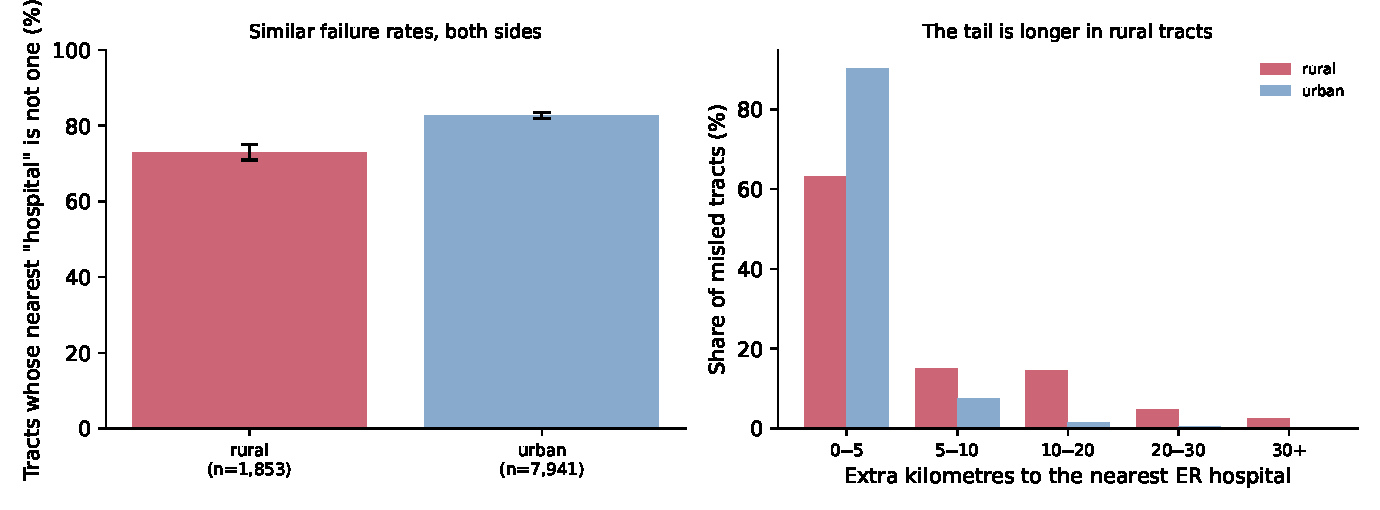
\includegraphics[width=0.92\textwidth]{figuras/hospital_error.pdf}
\caption{Left: the share of tracts whose nearest Overture ``hospital'' has no emergency
department is \emph{lower} in rural tracts (73.0\%) than in urban ones (82.6\%) --- the error
is not a rural phenomenon. Right: among misled tracts, how many extra kilometres separate the
Overture point from the real emergency department; the rural distribution has the heavier tail,
and within county that difference holds at 10\,km but not at 20\,km. Same mistake, different damage.}
\label{fig:hosp_err}
\end{figure}

\begin{itemize}
\item \textbf{21.5\%} [20.4, 22.6] of the \num{5561} ``hospital'' POIs are hospitals or
freestanding rooms with emergency services. Only 25.2\% are hospitals of any kind. Just 45.5\% are
something other than a clinic or a practice. The largest groups are clinics and practices (31.5\% of the
category) and uncategorised businesses (27.9\%).
\item The inflation is \textbf{6.6$\times$} overall --- \num{5561} POIs in the category
against the ER facilities the five regions are served by, as defined in the table --- and it
ranges from 3.6$\times$ in \texttt{eastern-wa} to 7.4$\times$ in \texttt{northern-ca}.
\item What the false positives are, as shares of all \num{5561} POIs (they total 71.2\%; the other
7.3 points of the 78.5\% are real hospitals without emergency services): 31.5\% clinics and practices,
27.9\% uncategorised businesses, 1.9\% urgent care, 1.7\% imaging and labs, 1.5\% behavioural health,
1.4\% administrative offices, 1.2\% wellness and spas, 4.0\% other.
\item Rural POIs are \emph{more} often real (32.9\% at level A against 20.4\% urban). The
category is noisiest where medical office parks are dense, which the precision figures show
but this study does not measure directly.
\item The same label does not mean the same thing across regions: precision runs from 14.4\%
in Maricopa to 27.0\% in Eastern Oklahoma and Eastern Washington ($\chi^2=\num{39.8}$,
$p=\num{4.8e-8}$). After Bonferroni, Maricopa differs from Eastern Oklahoma, South-Central Texas and Eastern
Washington, and Eastern Oklahoma from South-Central Texas.
\end{itemize}

\section{Who is misled, and how far}

\begin{table}[htbp]
\centering
\caption{Error and its tail by stratum, by region, and the Mantel--Haenszel odds ratios by
county. ``Error'' means the nearest Overture ``hospital'' has no emergency services; the
$\ge$10\,km columns count tracts where the real emergency department is at least that much
further away.}
\label{tab:severity}
\begin{adjustbox}{max width=\textwidth}
% Generated by procesos/bias_discovery/l9_hospitales.py
\begin{tabular}{@{}lrrrrrrr@{}}
\toprule
Stratum & Tracts & Error & $\geq$10 km & $\geq$20 km & $\geq$30 km & Pop. $\geq$10 km & Pop. $\geq$20 km \\
 & & \% & \% & \% & \% & \% & \% \\
\midrule
\multicolumn{8}{@{}l}{\emph{Error and its tail, by stratum}} \\
all tracts & 9794 & 80.8 & 4.5 & 1.6 & 0.6 & 3.9 & 1.2 \\
\quad rural & 1853 & 73.0 & 16.1 & 5.4 & 1.8 & 16.3 & 4.6 \\
\quad urban & 7941 & 82.6 & 1.8 & 0.7 & 0.3 & 1.6 & 0.5 \\
\quad tribal & 935 & 70.8 & 8.1 & 3.3 & 1.3 & 7.5 & 2.6 \\
\quad non-tribal & 8859 & 81.9 & 4.1 & 1.4 & 0.5 & 3.6 & 1.0 \\
\quad SVI high & 3362 & 80.2 & 5.4 & 2.1 & 0.9 & 5.1 & 1.7 \\
\quad SVI low & 1900 & 83.6 & 1.8 & 0.3 & 0.1 & 1.4 & 0.1 \\
\midrule
\multicolumn{8}{@{}l}{\emph{By region}} \\
\quad maricopa-az & 1593 & 88.1 & 4.0 & 2.0 & 0.8 & 3.0 & 1.2 \\
\quad northern-ca & 591 & 79.5 & 6.3 & 1.7 & 0.3 & 5.1 & 1.4 \\
\quad eastern-ok & 1192 & 68.2 & 4.8 & 1.4 & 0.4 & 4.6 & 1.1 \\
\quad south-central-tx & 6003 & 82.1 & 4.5 & 1.4 & 0.5 & 4.0 & 1.1 \\
\quad eastern-wa & 415 & 72.5 & 4.1 & 1.9 & 1.0 & 3.8 & 1.5 \\
\midrule
\multicolumn{8}{@{}l}{\emph{Lower-bound reference, distance only: any acute, CAH, REH, VA, DoD or freestanding hospital, whatever the flag}} \\
\quad rural & 1853 & 73.0 & 16.1 & 5.4 & -- & 16.3 & -- \\
\quad urban & 7941 & 82.6 & 1.8 & 0.7 & -- & 1.6 & -- \\
\midrule
\multicolumn{8}{@{}l}{\emph{Mantel--Haenszel odds ratio by county, case = error and extra kilometres above threshold}} \\
\multicolumn{8}{@{}l}{\quad \emph{Stratum} \hfill \emph{n} \hspace{1.2cm} \emph{OR} \hspace{1.1cm} \emph{95\% CI} \hspace{1.1cm} \emph{bootstrap}} \\
\quad rural, any error & 9756 & 1.02 & [0.87, 1.20] & [0.82, 1.28] \\
\quad rural, $\geq$10 km & 9756 & 2.86 & [2.11, 3.88] & [2.00, 4.30] \\
\quad rural, $\geq$20 km & 9756 & 1.02 & [0.64, 1.62] & [0.47, 2.09] \\
\quad rural, $\geq$30 km & 9756 & 0.77 & [0.34, 1.73] & [0.11, 3.11] \\
\quad rural, extra/real $\geq$0.5 & 9756 & 0.37 & [0.31, 0.45] & [0.29, 0.46] \\
\quad rural, conservative floor & 9756 & 1.02 & [0.89, 1.18] & [0.85, 1.23] \\
\quad rural, $\geq$10 km, region $\times$ density & 9794 & 12.50 & [8.15, 19.18] & [9.53, 17.87] \\
\quad rural, $\geq$10 km, lower bound reference & 9756 & 2.89 & [2.13, 3.92] & [2.01, 4.33] \\
\quad rural, $\geq$20 km, lower bound reference & 9756 & 0.99 & [0.62, 1.56] & [0.46, 2.00] \\
\quad tribal, $\geq$10 km & 9756 & 3.25 & [1.48, 7.15] & [1.57, 9.14] \\
\quad SVI high, $\geq$10 km & 5214 & 1.52 & [0.95, 2.43] & [0.80, 3.09] \\
\bottomrule
\multicolumn{8}{@{}p{14.6cm}@{}}{\footnotesize Bootstrapped by resampling counties with replacement (2,000 draws, seed 42); counties are the strata of the Mantel--Haenszel estimate. Extra kilometres are straight-line, from the tract centroid to the nearest ER hospital minus the distance to the nearest Overture ``hospital'' POI, floored at zero. Conservative floor: every POI whose name suggests a hospital (hospital, medical center, health system, military) counts as real. Extra/real: extra kilometres divided by the distance to the real ER.} \\
\end{tabular}

\end{adjustbox}
\end{table}

\begin{itemize}
\item In \textbf{80.8\%} of the \num{9794} tracts, the nearest Overture ``hospital'' has no
emergency services. Those tracts hold \textbf{32,973,353 of 40,427,337 residents (81.6\%)}.
\item The mean penalty is \textbf{2.38\,km} of straight-line distance (rural 4.47\,km, urban
1.90\,km), \textbf{2.24\,km} weighted by population, and \textbf{2.92\,km} over the affected tracts
only (\textbf{2.72\,km} when those are weighted by population).
\item The disparity is in the tail, not the rate, and it sits between 10 and 20\,km. Tracts where
the real ER is at least 10\,km beyond the Overture point: \textbf{16.1\% rural (298 tracts) against
1.8\% urban (145)}, Mantel--Haenszel odds ratio by county \textbf{2.86 [2.11, 3.88]}, bootstrap
[2.00, 4.30]; with the generous reference, 2.89 [2.13, 3.92]. Stratifying by region $\times$
POI-density tertile instead of by county raises it to \textbf{12.50 [8.15, 19.18]}: the county
absorbs part of the rurality, so the within-county estimate is the conservative one.
\item \textbf{The result survives an incomplete reference.} No registry lists hospitals' off-campus
emergency departments, so the base reference still misses some, mostly in metropolitan areas. Two stress tests
(\path{procesos/bias_discovery/l9_sensibilidad_ref.py}) measure the effect. Treating the 91
licences from the 2020 Texas list that are absent from today's roster as still open gives 2.91
[2.23, 3.80]. Counting as a real ER every one of the \num{1215} health POIs in Overture whose name
presents it as one, an overcount, gives 12.7\% rural against 1.0\% urban and 3.33
[2.40, 4.62].
\item Tribal tracts: 8.1\% at $\ge$10\,km against 4.1\% non-tribal, OR 3.25 [1.48, 7.15], on few
counties, so the interval is wide.
Here ``tribal'' is \texttt{tribal\_pct}$>0$ from the strata table, \num{935} tracts; the
stricter \texttt{tribal\_any} flag gives \num{874} tracts.
\item \textbf{What does not hold:} the probability of error is \emph{not} higher in rural
tracts (OR 1.02 [0.87, 1.20]); the conservative floor gives 1.02 [0.89, 1.18]; at $\ge$20\,km
the rural OR is 1.02 [0.64, 1.62], and even the overcounting test gives 1.50 [0.89, 2.53], neither
significant; at $\ge$30\,km it is 0.77 [0.34, 1.73]. Social vulnerability is unsettled: high-SVI
tracts are no more likely to be misled (OR 0.83 [0.69, 1.00]) and the $\ge$10\,km estimate is 1.52
[0.95, 2.43]. The $\ge$20\,km estimate is 3.86 [1.04, 14.27], too wide to rely on, and these estimates moved
when the reference changed (the $\ge$10\,km estimate was 0.91 before the freestanding list was added).
\end{itemize}

\noindent Every distance here is centroid-to-point Euclidean in EPSG:5070, \textbf{not travel time}. What the
straight-line number establishes is \emph{ordering}: the Overture point is systematically closer than the
emergency department, and the gap grows in rural tracts. Road distance was not computed.

Filtering by \texttt{confidence} does not repair the layer. Restricting to POIs with
\texttt{confidence}$\ge0.90$ leaves \num{2545} points, raises precision A to 28.9\%, and still
leaves 73.2\% of tracts misled, against 80.8\% unfiltered. The one odds ratio in that filter
(0.94 [0.80, 1.09]) is the \emph{probability} of being misled by the nearest high-confidence
POI, rural against urban by county: it says rural tracts are not more likely to be wrong when
low-confidence points are removed, not that the tail improves --- the filter drops rural POIs
wholesale. The field measures how sure Overture is that a place exists, not what it is.

\section{The places}

\begin{table}[htbp]
\centering
\caption{Eight rural places where the nearest Overture ``hospital'' is not a hospital with
emergency services. All rows verified on the web on 31 October 2026.}
\label{tab:rural}
\makeatletter
\def\input@path{{tablas/}}
\makeatother
\begin{adjustbox}{max width=\textwidth}
\begingroup\catcode`\/=\active\def/{\char`/\allowbreak}%
\input{hospital_rural.tex}
\endgroup
\end{adjustbox}
\end{table}

\begin{table}[htbp]
\centering
\caption{Six verified tracts from the ranking by population $\times$ extra kilometres; three are
urban and three rural by the 50\% rule.}
\label{tab:urban}
\begin{adjustbox}{max width=\textwidth}
% Generated by procesos/bias_discovery/l9_hospitales.py
{\footnotesize
\begin{tabular}{@{}p{1.8cm}p{2.2cm}p{2.1cm}rp{4.3cm}p{3.4cm}rr@{}}
\toprule
Place & County & Census tract & Pop. & Nearest Overture ``hospital'' & Nearest real ER hospital & POI (km) & ER (km) \\
\midrule
Hockley area & Harris, TX & 48201556000 CT 5560 & 12,481 & Memorial Herman Daikin Facitily [other, no keyword] & FAIRFIELD EMERGENCY ROOM & 2.6 & 14.6 \\
East Midland & Midland, TX & 48329010123 CT 101.23 & 12,127 & Medcor Clinic at Pioneer Natural Resources [clinic or practice] & MIDLAND MEMORIAL HOSPITAL & 3.6 & 11.2 \\
Luckey Ranch & Bexar, TX & 48029161902 CT 1619.02 & 15,735 & Luckey Ranch - University Health [school or training] & PHYSICIANS PREMIER & 6.8 & 12.4 \\
Rio Rico & Santa Cruz, AZ & 04023966108 CT 9661.08 & 6,249 & Free STD Clinics [other, no keyword] & HOLY CROSS HOSPITAL & 1.6 & 13.4 \\
Aldine & Harris, TX & 48201222900 CT 2229 & 8,030 & HCHD Aldine Health Clinic [clinic or practice] & MEMORIAL HERMANN NORTHEAST HOSPITAL & 2.6 & 11.3 \\
Natomas & Sacramento, CA & 06067007106 CT 71.06 & 7,378 & Vortran Medical Technology 1, Inc. [clinic or practice] & SUTTER MEDICAL CENTER, SACRAMENTO & 2.3 & 11.1 \\
\bottomrule
\multicolumn{8}{@{}p{14.6cm}@{}}{\footnotesize Distances are straight-line from the tract centroid, not travel time. Sorted by population $\times$ extra kilometres. Each row was checked on the web on 31 October 2026. In row order: Hockley area: an HVAC factory (the Daikin Texas Technology Park) in unincorporated Harris County near Waller, https://daikintexastechnologypark.com/page/contact ; ER: Fairfield Emergency Room, Cypress; Luckey Ranch: a walk-in primary-care clinic in the Luckey Ranch subdivision off US 90, https://www.universityhealth.com/locations/luckey-ranch ; ER: Physicians Premier, Potranco Road; East Midland: an on-site occupational-health clinic at Pioneer Natural Resources' Midland offices, https://medcor.com/clinics/ ; ER: Midland Memorial Hospital; Rio Rico: a directory listing in a commercial strip, 54 m from Mariposa Community Health Center, https://mariposachc.net/locations/ ; ER: Holy Cross Hospital, a critical access hospital (CMS Hospital General Information); Aldine: a Harris Health primary-care clinic on Aldine Mail Route, closed at weekends, https://www.harrishealth.org/locations-hh/Pages/aldine-health-center.aspx ; ER: Memorial Hermann Northeast Hospital; Natomas: a medical-device manufacturer in the Natomas industrial area, https://www.vortran.com/ ; ER: Sutter Medical Center.} \\
\end{tabular}}

\end{adjustbox}
\end{table}

Every row was checked for what the Overture point is and for any hospital or emergency room closer
than the one listed. The tract holding \textbf{Zapata, Texas} (\num{2567} residents): the nearest
``hospital'' is a community health centre whose own page says ``This is not an emergency clinic'';
the nearest emergency department is in Laredo, 61.7\,km from the centroid.
\textbf{Freer} (tract of \num{2887}): an outpatient clinic closed at weekends, 2.9\,km away; the
ER is 60.5\,km away in Alice. \textbf{Falfurrias} (\num{2236}): 62.6\,km to Kingsville.
\textbf{Post} (\num{2901}): the nearest ``hospital'' is a scout camp, and the ER is 48.0\,km away in
Tahoka.
\textbf{Gila Bend, Arizona} (\num{2486}): a directory listing located in a truck-stop plaza on I-8,
71.6\,km from the standalone Abrazo Buckeye Emergency Center. \textbf{Ajo} (\num{3207}): a dental
clinic in another tract, 107.4\,km from the Sells hospital. \textbf{Salome} (\num{1028}): a family
clinic, 90.0\,km from Wickenburg Community Hospital. \textbf{Holbrook} (\num{3498}): 62.7\,km from
Little Colorado Medical Center. That is \num{20810} residents across these eight tracts, every one
of them with a mapped ``hospital'' that is not a hospital. Two of the Arizona tracts are large and
mostly empty (\num{1319} and \num{3974}\,km$^2$), so their centroids lie some 20 to 30\,km from the
settlement that names them; distances are centroid-to-point as everywhere else, and the aggregate
statistics do not rest on these rows.

Table~\ref{tab:urban} comes from a ranking of tracts by population $\times$ extra kilometres. Of the top fifteen in
an earlier run, nine fell because an off-campus hospital emergency department sits closer; those departments
then entered the reference, and tracts that rose in the ranking afterwards were not checked individually. The
six that passed include an HVAC factory in Harris County and a medical-device manufacturer in Sacramento, with
5.6 to 12.0\,km of extra distance. The Luckey Ranch POI is a walk-in clinic; the classifier tags it as school
or training because of the word ``University'' in its name.

\section{Why it matters for dispatch and relief}

The organiser's own framing is that these data support emergency dispatch, evacuation routing
and disaster relief. A dispatch or relief tool that answers ``nearest hospital'' from this
layer sends an ambulance, a family or a relief team to a clinic, a dental office or a scout
camp. In the eight tracts above, the nearest emergency department is 48 to 107\,km from the
tract centroid, against 2.9 to 52.8\,km for the Overture point. Three sources frame the consequence:

\begin{enumerate}
\item \textbf{The regulatory baseline.} 42 CFR 485.618(a) requires that a Critical Access
Hospital make emergency services available 24 hours a day; 42 CFR 485.618(d) requires a
clinician with emergency training on call, immediately available by telephone or radio, and on
site within 30 minutes (60 in approved frontier areas). A facility
that does not meet this is not a substitute for an ER, however medical its name.
\item \textbf{Closures and the substitute provider type.} CMS states that Rural Emergency
Hospitals were created under the Consolidated Appropriations Act 2021 ``to respond to rural
hospital closures'' and that an REH must provide emergency department services and comply with
EMTALA. Rural closures are frequent enough to have generated a dedicated provider category;
each closure moves the nearest ER further away, which is exactly the quantity our table
measures.
\item \textbf{Time.} Predicted travel time above 30 minutes to a trauma centre was associated
with a 66\% higher adjusted risk of death for motor-vehicle trauma (OR 1.66, 95\% CI
1.09--2.52) and a 3.4-fold risk for penetrating trauma (OR 3.43, 1.37--8.59) in a
population-based cohort of \num{1535} patients. The motor-vehicle association disappears when
scene deaths are excluded (OR 0.93, 0.58--1.46). The cohort is Canadian and blunt-trauma dominant,
so it serves as an order of magnitude: a 30-minute boundary can be clinically meaningful. Its threshold is
travel \emph{time}, while our figure is straight-line \emph{distance}.
\end{enumerate}

\section{Limitations}

\begin{itemize}
\item \textbf{Some ``hospitals'' are useful places.} An urgent care, a dialysis unit or a rural health clinic
is a real service; it is not an emergency department, and a nearest-facility query returns it as if it were.
Level C shows how much survives that weaker reading (45.5\%).
\item \textbf{The reference is incomplete.} Hospitals' off-campus emergency departments appear in
no registry, Arizona's list covers the central region and some of Pima County, and 20 CMS facilities
have no coordinates; 25 sit at their city's centroid. Geocoding mixes Census and OpenStreetMap, so individual
distances can be off by a few kilometres: East Midland reads 11.2\,km here and 10.6\,km against a Census geocode
of the same hospital. Each named place was checked individually against web sources.
\item \textbf{CMS's flag has errors of its own.} A psychiatric hospital in Sacramento carries
emergency services ``Yes''; single records were not corrected.
\end{itemize}

\section{Recommendation}

\begin{enumerate}
\item \textbf{Publish precision by category alongside the score.} A single number per
category --- share of POIs that are the thing the category names --- costs nothing to compute
and would have exposed this layer before anyone used it for routing.
\item \textbf{Add a precision metric to the Bias Score.} The five existing metrics all measure
shortage. A sixth, computed as the share of a category's POIs that survive a name-and-location
match against a public registry, measures the opposite failure and is the only way the
scorecard can see a map that over-counts.
\item \textbf{Do not exclude a category because it cannot show a deficit; score its error
rate.} Exclusion is the mechanism that created the blind spot.
\end{enumerate}

\section{Supporting finding: care centres are missing in the same direction}

The mirror-image test is a category that \emph{should} show a deficit and does. Nursing homes,
dialysis units and federally qualified health centres in the five regions were matched to CMS
certified facilities (\num{3384} centres after removing \num{172} opened after 2025-01-01, so
that Overture's 2026-08-19 snapshot is not blamed for facilities that did not exist).

\begin{table}[htbp]
\centering
\caption{Absence rates for care centres, by type, region and rurality, with the
Mantel--Haenszel odds ratio by county and the density-adjusted version.}
\label{tab:care_rates}
\begin{adjustbox}{max width=\textwidth}
% Generated by procesos/bias_discovery/l7_cuidado.py
\begin{tabular}{@{}lrrrr@{}}
\toprule
Stratum & $n$ & 1-km rule & Name rule & 95\% CI (name rule) \\
\midrule
\multicolumn{5}{@{}l}{\emph{By centre type}} \\
\quad dialysis & 780 & 1.7 & 1.4 & [0.8, 2.5] \\
\quad health center & 1093 & 4.7 & 4.2 & [3.2, 5.6] \\
\quad nursing home & 1511 & 7.5 & 3.2 & [2.4, 4.2] \\
\midrule
\multicolumn{5}{@{}l}{\emph{By region}} \\
\quad maricopa-az & 419 & 3.3 & 2.6 & [1.5, 4.6] \\
\quad northern-ca & 261 & 2.7 & 1.9 & [0.8, 4.4] \\
\quad eastern-ok & 514 & 8.9 & 5.4 & [3.8, 7.8] \\
\quad south-central-tx & 1992 & 4.9 & 2.7 & [2.1, 3.5] \\
\quad eastern-wa & 198 & 6.1 & 3.5 & [1.7, 7.1] \\
\midrule
\multicolumn{5}{@{}l}{\emph{Rural vs urban, overall and by type}} \\
\quad all centers --- rural & 550 & 10.0 & 6.4 & [4.6, 8.7] \\
\quad all centers --- urban & 2834 & 4.3 & 2.5 & [2.0, 3.1] \\
\quad dialysis --- rural & 30 & 10.0 & 3.3 & [0.6, 16.7] \\
\quad dialysis --- urban & 750 & 1.3 & 1.3 & [0.7, 2.4] \\
\quad health center --- rural & 220 & 8.2 & 8.2 & [5.2, 12.6] \\
\quad health center --- urban & 873 & 3.8 & 3.2 & [2.2, 4.6] \\
\quad nursing home --- rural & 300 & 11.3 & 5.3 & [3.3, 8.5] \\
\quad nursing home --- urban & 1211 & 6.5 & 2.6 & [1.9, 3.7] \\
\midrule
\multicolumn{5}{@{}l}{\emph{Rural vs urban Mantel--Haenszel odds ratio}} \\
\quad \emph{Stratum} & $n$ & \multicolumn{2}{r}{\emph{Bootstrap CI}} & \emph{OR [MH 95\% CI]} \\
\quad overall & 3346 & \multicolumn{2}{r}{[1.80, 4.76]} & 2.94 [1.48, 5.82] \\
\quad overall, name rule & 3346 & \multicolumn{2}{r}{[2.83, 12.58]} & 5.55 [1.95, 15.75] \\
\quad nursing home & 1446 & \multicolumn{2}{r}{[1.13, 4.35]} & 2.25 [0.96, 5.28] \\
\quad dialysis & 703 & \multicolumn{2}{r}{[8.17, 190.29]} & 22.56 [0.00, 594384.40] \\
\quad health center & 1023 & \multicolumn{2}{r}{[0.77, 7.60]} & 2.42 [0.73, 8.07] \\
\quad nursing home, name rule & 1446 & \multicolumn{2}{r}{[1.65, 22.24]} & 4.68 [1.09, 20.08] \\
\quad dialysis, name rule & -- & \multicolumn{2}{r}{not identified} & -- \\
\quad health center, name rule & 1023 & \multicolumn{2}{r}{[1.47, 17.52]} & 4.48 [0.79, 25.29] \\
\quad eastern-ok, name rule & 505 & \multicolumn{2}{r}{[3.80, 43.24]} & 10.67 [1.12, 102.09] \\
\quad south-central-tx, name rule & 1966 & \multicolumn{2}{r}{[2.41, 31.47]} & 7.54 [1.04, 54.57] \\
\quad maricopa-az, name rule & 419 & \multicolumn{2}{r}{[1.21, 48.21]} & 6.00 [0.17, 214.11] \\
\quad northern-ca, name rule & 259 & \multicolumn{2}{r}{[0.30, 2.66]} & 0.89 [0.01, 68.21] \\
\quad eastern-wa, name rule & 197 & \multicolumn{2}{r}{[0.28, 5.70]} & 1.29 [0.18, 9.44] \\
\quad density-adjusted & 3378 & \multicolumn{2}{r}{[0.40, 1.71]} & 1.49 [0.85, 2.64] \\
\quad false-negative corrected & 3346 & \multicolumn{2}{r}{[2.81, 12.46]} & 5.49 [1.91, 15.77] \\
\bottomrule
\multicolumn{5}{@{}p{13.5cm}@{}}{\footnotesize Dialysis rests on very few rural cases, so its intervals are unstable and are reported as computed.} \\
\end{tabular}

\end{adjustbox}
\end{table}

\begin{itemize}
\item \textbf{5.2\%} of centres have no POI matching them by name within 1\,km and no care-category
POI within 100\,m (177 of \num{3384}); with a name rule
that accepts a near-identical name within 6\,km, \textbf{3.1\%} (105) are missing.
\item Rural against urban, \emph{1-km rule}: 10.0\% against 4.3\%, MH odds ratio by county
\textbf{2.94 [1.48, 5.82]}.
\item Rural against urban, \emph{name rule}: 6.4\% against 2.5\%, MH odds ratio
\textbf{5.55 [1.95, 15.75]}.
\item That name-rule estimate stratified by POI-density tertile instead of by county drops to
\textbf{1.49 [0.85, 2.64]} ($n=\num{3378}$): this is a general property of sparse mapping, not
something specific to care.
\item The 105 missing centres carry \textbf{4,786 certified nursing-home beds} and
\textbf{3,077 residents per day}, plus \textbf{206 dialysis stations} serving \textbf{737}
one-year dialysis patients. Units are not summed.
\end{itemize}

\begin{table}[htbp]
\centering
\caption{Fifteen of the missing care centres, largest first, with the nearest Overture POI and
its category: a jerky shop, a nail salon, a gravel yard and a post office stand in for nursing
homes and dialysis units.}
\label{tab:care_missing}
\begin{adjustbox}{max width=0.9\textwidth}
% Generated by procesos/bias_discovery/l7_cuidado.py
\begin{tabular}{@{}p{4.1cm}p{3.0cm}p{1.9cm}lp{3.4cm}rrrr@{}}
\toprule
Center & Census tract & County & Type & Nearest Overture POI & Dist. & Beds & Stat. & Res. \\
 & & & & & (m) & & & /day \\
\midrule
CEDAR HOLLOW REHABILITATION CENTER & 48181001801 (Census Tract 18.01) & Grayson (TX) & nursing home & XPO [business to business] & 270 & 142 & -- & 122 \\
WILLOW PARK REHABILITATION AND CARE CENTER & 48367140604 (Census Tract 1406.04) & Parker (TX) & nursing home & Lone Star Jerky [restaurant] & 99 & 125 & -- & 85 \\
ROYSE CITY MEDICAL LODGE & 48231961401 (Census Tract 9614.01) & Rockwall (TX) & nursing home & McLarry Sand and Gravel [building supply store] & 248 & 124 & -- & 87 \\
Medina Valley Health \& Rehabilitation Center & 48029161902 (Census Tract 1619.02) & Medina (TX) & nursing home & Pagel's Resale Shop [discount store] & 362 & 116 & -- & 85 \\
Avir at Caldwell & 48051970202 (Census Tract 9702.02) & Burleson (TX) & nursing home & Burleson County Historical Museum [museum] & 96 & 112 & -- & 48 \\
Avir at Pittsburg & 48063950102 (Census Tract 9501.02) & Camp (TX) & nursing home & Thunderbird Point Owners Association [community services non profits] & 527 & 102 & -- & 46 \\
Cedar Lake Nursing Center & 48213951000 (Census Tract 9510) & Henderson (TX) & nursing home & Mel’s Nails \& Foot Spa [hair salon] & 123 & 90 & -- & 52 \\
CROCKETT HEALTH CARE ASSOCIATES, INC. & 48225950200 (Census Tract 9502) & Houston (TX) & nursing home & Porter Springs Baptist Church [baptist church] & 161 & 90 & -- & 40 \\
Calera Manor & 40013796600 (Census Tract 7966) & Bryan (OK) & nursing home & United States Postal Service [post office] & 208 & 82 & -- & 78 \\
COMMUNITY HEALTH CARE OF GORE & 40135030202 (Census Tract 302.02) & Sequoyah (OK) & nursing home & Styles + Sets by Stormi [spas] & 51 & 70 & -- & 40 \\
MRC CREEKSIDE & 48471790301 (Census Tract 7903.01) & Walker (TX) & nursing home & Creekside Retirement Community [retirement home] & 303 & 66 & -- & 42 \\
QUIBURI MISSION NURSING \& REHABILITATION & 04003000305 (Census Tract 3.05) & Cochise (AZ) & nursing home & Turquoise Hills by Century Complete [builders] & 74 & 60 & -- & 53 \\
DaVita Mid Columbia Kidney Center & 53021020608 (Census Tract 206.08) & Franklin (WA) & dialysis & Market North Co. [home goods store] & 364 & -- & 22 & 74 \\
Central Oklahoma Family Medical Center - Primary 1/Wound/Podiatry & 40123088700 (Census Tract 887) & Pontotoc (OK) & health center & Susmita Sakruti, M.D. [oncologist] & 334 & -- & -- & -- \\
Human Services and Child Welfare & 06093001300 (Census Tract 13) & Siskiyou (CA) & health center & Karuk Senior Nutrition Program [social and human services] & 80 & -- & -- & -- \\
\bottomrule
\multicolumn{9}{@{}p{13.5cm}@{}}{\footnotesize Beds: Medicare/Medicaid-certified nursing-home beds (CMS 4pq5-n9py). Stat.: dialysis stations (CMS 23ew-n7w9). Res./day: average residents per day for nursing homes, one-year Medicare dialysis patients for dialysis units. Units are not summed.} \\
\end{tabular}

\end{adjustbox}
\end{table}

\begin{figure}[htbp]
\centering
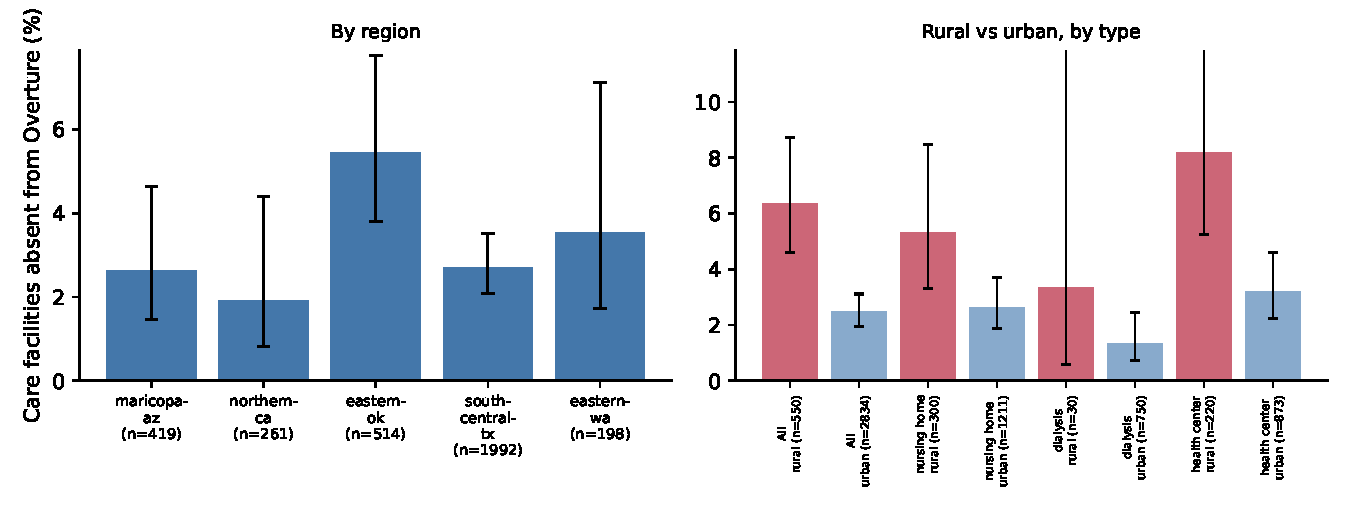
\includegraphics[width=0.76\textwidth]{figuras/care_rates.pdf}
\caption{Absence of care facilities from Overture under the name rule, by region (left) and by centre type for
rural against urban tracts (right). The disparity is largely explained by POI density.}
\label{fig:care}
\end{figure}

A category the score \emph{includes} (care centres, via the
establishments half) shows a modest deficit that the POI-density tertiles largely explain. A
category the score \emph{excludes} (hospitals) hides a 78.5\% error rate that nothing in the
challenge measures. The contrast is exclusion, not scarcity: both categories miss facilities,
but only the excluded one misses them in the other direction and goes unaudited.

\section{Hypotheses tested and rejected}

Seven candidate discoveries were tested and abandoned.

\noindent\begin{minipage}{\textwidth}
\small
\captionof{table}{Hypotheses that did not survive their own test.}
\label{tab:rejected}
\begin{tabular}{@{}>{\raggedright\arraybackslash}p{3.2cm}>{\raggedright\arraybackslash}p{4.9cm}>{\raggedright\arraybackslash}p{4.8cm}@{}}
\toprule
Hypothesis & What we measured & Why it fails \\
\midrule
Post-fire rebuilt areas have a coverage gap (Butte County 2018) & Overture detects
\textbf{92.2\%} of the structures that still stand; the apparent deficit of \num{4194}
buildings against \num{16386} destroyed is the fire & The ``gap'' is destruction, not mapping \\
Building gap is an artefact of the upstream source & Within county the effect collapses to
$+\num{0.015}$; CarbonPlan buildings correlate \num{0.9996} with Overture, USFS \num{0.97} &
Neither layer is an independent reference, so the ``comparison'' is Overture against itself \\
Tribal nations are systematically under-mapped & 10 county-level tests across the large
Oklahoma nations, Holm-corrected & \textbf{0 of 10} survive correction \\
Texas colonias are the intersection the strata miss & Border-county colonia tracts against
matched non-colonia tracts & Adjusted effect $+\num{0.193}$ with the \emph{opposite} sign to
the hypothesis \\
Evacuation egress: unnamed or low-class boundary crossings grow with wildfire risk & 4 cells
by egress class, with a track/service control & After removing track/service, 1 of 4 cells
survives; the Paradise control fails \\
Mobile-home share marks under-mapping & $+\num{0.324}$ [0.243, 0.462] on building count &
Those tracts have \emph{more} buildings, not fewer: the sign is against a deficit \\
New subdivisions (share built 2020+) are under-mapped & $+\num{0.005}$, $p=0.98$ &
No effect \\
\bottomrule
\end{tabular}
\end{minipage}

\section{Reproducing the finding}

\begin{verbatim}
pip install -r requirements.txt
# challenge data, no account needed, into CONCURSO/data/<same paths as the bucket>:
#   https://data.source.coop/humane-intelligence/bias-bounty-mapping-equity-challenge/
#   strata/national/national-strata-tract-table.parquet
#   strata/<region>/<region>-census-tracts.parquet
#   reference/<region>/<region>-overture-pois.parquet
export PYTHONIOENCODING=utf-8
python procesos/bias_discovery/l9_hospitales.py
python procesos/bias_discovery/l9_sensibilidad_ref.py
python procesos/bias_discovery/l7_cuidado.py
\end{verbatim}

The finding has two script sets: \path{procesos/bias_discovery/l9_*.py} classifies hospitals
(\path{l9_hospitales.py} classification, \path{l9_referencia.py} reference and geocoding,
\path{l9_geo_respaldo.py} the OpenStreetMap fallback, \path{l9_salidas.py} tables and figure,
\path{l9_sensibilidad_ref.py} the reference tests) and \path{procesos/bias_discovery/l7_cuidado.py}
does the care-centre match. External records and their geocoding caches sit in
\path{datos/externos/}, so no network call is needed except for DuckDB's \texttt{spatial}
extension. The run also reads \path{datos/features_base/features_buildings.parquet}, in the repository,
to fix the 9,794 scored GEOIDs. CSV outputs go to \path{datos/bias_discovery/}; tables and figures to
\path{docs/2_premios/writeup/}. Running \path{l9_hospitales.py} twice gave the same CSVs and tables;
the PDF figures differ only in metadata across Matplotlib versions. All resampling uses
\texttt{seed=42}: \texttt{random\_state=42} for the three validation samples and \texttt{seed=42} for
the 2,000-draw county bootstrap. Ties in the POI-density tertiles are broken by GEOID.

\noindent\footnotesize Additional sources, retrieved 30--31 October 2026, with dated copies in
\path{datos/externos/}. US federal records are public domain; state records are published public records:
\begin{sloppypar}
\begin{itemize}\footnotesize
\item CMS Hospital General Information, \url{https://data.cms.gov/provider-data/dataset/xubh-q36u}
\item CMS nursing-home provider information, \url{https://data.cms.gov/provider-data/dataset/4pq5-n9py}; dialysis facilities, \url{https://data.cms.gov/provider-data/dataset/23ew-n7w9}
\item VA VHA facilities, \url{https://services1.arcgis.com/smmmD7AGkh7eJR2a/arcgis/rest/services/Veterans_Health_Administration_(VHA)_Facilities/FeatureServer/0}; IHS health facilities, \url{https://services2.arcgis.com/VFLAJVozK0rtzQmT/arcgis/rest/services/ITU_Health_Facilities_All_Fields_View/FeatureServer/0}
\item Texas HHSC freestanding emergency medical care roster, \url{https://www.hhs.texas.gov/sites/default/files/documents/doing-business-with-hhs/provider-portal/facilities-regulation/freestanding-emergency/femc-directory.xlsx} (cut 2026-10-21); Texas DSHS 2020 list, used only in the sensitivity test
\item Arizona AEMS categorisation status report, \url{https://aems.org/images/pdf/categorization/categorization-status-report-current.pdf} (2026-10-19); Oklahoma OSDH directory of medical facilities, \url{https://www.oklahoma.gov/content/dam/ok/en/health/health2/aem-documents/protective-health/medical-facilities-division/mfs-directoryoffacilities.pdf} (2026-07-08); per-row operator pages in \path{fsed_referencia.csv}
\item OpenStreetMap Nominatim, \url{https://nominatim.openstreetmap.org/} (ODbL), for 236 CMS addresses the Census Geocoder did not resolve
\item US Census county FIPS names, \url{https://www2.census.gov/geo/docs/reference/codes/files/national_county.txt}
\item 42 CFR 485.618, \url{https://www.ecfr.gov/current/title-42/part-485/section-485.618} (emergency services 24 h a day; clinician on site within 30 min)
\item CMS, Rural Emergency Hospitals, \url{https://www.cms.gov/medicare/health-safety-standards/certification-compliance/rural-emergency-hospitals} (created ``to respond to rural hospital closures'')
\item Tansley G. \emph{et al.}, Predicted travel time to trauma care and mortality, \emph{Can J Surg} 2019;62(2):123--130, \url{https://pmc.ncbi.nlm.nih.gov/articles/PMC6440889/}
\end{itemize}
\end{sloppypar}


\end{document}
